



\begin{table}[ht]
\centering
\caption{Statistics of datasets. FB means FreeBase.}
\small
\label{tab:dataset_statistics}
\begin{tabular}{|c|c|c|c|c|}
\hline
\textbf{Dataset} & \textbf{ExplaGraphs} & \textbf{SceneGraphs} & \textbf{WebQSP}  \\ \hline
\#Graphs          & 2,766               & 100,000             & 4,737                    \\ \hline
Average \#Nodes   & 5.17                & 19.13               & 1370.89                  \\ \hline
Average \#Edges   & 4.25                & 68.44               & 4252.37                 \\ \hline
Node Attribute    &  concepts & Object attributes    & Entities in FB  \\ \hline
Edge Attribute    &  relations & Spatial relations   & Relations in FB  \\ \hline
Task              &  reasoning & Scene graph QA       & KGQA             \\ \hline
Evaluation metrics & Accuracy            & Accuracy            & Hit@1              \\ \hline
\end{tabular}
\end{table}


\begin{table*}[ht]
\centering
\caption{Performance comparison for different methods (\%).}
\vspace{-0.7\baselineskip}  % Tighter vertical spacing
\small
\label{tab:performance_comparison_A_side}
\begin{tabular}{|c|c|c|c|}
\hline
\textbf{Dataset (Metrics)} & \textbf{ExplaGraphs (ACC)} & \textbf{SceneGraphs (ACC)} & \textbf{WebQSP (Hit@1)} \\ \hline
Zero-shot                   & 56.50                      & 39.74                      & 41.06                    \\ 
Zero-CoT (Kojima et al., 2022) & 57.04                  & 52.60                      & 51.30                    \\ 
CoT-BAG (Wang et al., 2024)  & 57.94                      & 56.80                      & 39.60                    \\ 
KAPING (Baek et al., 2023)   & 62.27                      & 43.75                      & 52.64                    \\ 
Graph-based Inference        & 33.93                      & 42.17                      & 47.22                    \\ 
Frozen LLM + Prompt Tuning (PT) & 58.98                  & 63.72                      & 54.11                    \\ 
GraphToken (Perozzi et al., 2024) & 85.08               & 49.03                      & 57.05                    \\ 
G-Retriever                  & 86.19                      & 80.86                      & 70.02                    \\ \hline
\myModel\                    & 87.31                      & 82.32                      & 71.36                    \\ \hline
\end{tabular}
\label{result_table}
\vspace{-1.3\baselineskip}  % Tighter vertical spacing
\end{table*}

\noindent\textbf{Datasets.}  
We evaluate on the GraphQA benchmark~\cite{gretriever}, which includes ExplaGraphs, SceneGraphs, and WebQSP. Dataset stats are in Table~\ref{tab:dataset_statistics} in the Appendix.
\noindent\textbf{Metrics.}  
Following GRetriever, we use accuracy for ExplaGraphs and SceneGraphs, and Hit@1 for WebQSP, which allows multiple correct answers.
\noindent\textbf{Baselines.}  
We compare against inference-only methods (e.g., Zero-shot ~\cite{zeroshot}, CoT-BAG~\cite{CoT-BAG}, KAPING~\cite{KAPING}) and prompt-tuning methods (e.g., Prompt Tuning, GraphToken~\cite{GraphToken}, G-Retriever~\cite{gretriever}).


% \noindent\textbf{Datasets.}  
% We evaluate our approach using the GraphQA benchmark~\cite{}, which contains three datasets: ExplaGraphs, SceneGraphs, and WebQSP. Summary statistics are presented in Table~\ref{}. Additional details about each dataset are provided in the Appendix.


% \noindent\textbf{Metrics.}  
% We follow the experimental setup of GRetreiver ~\cite{} and adopt the evaluation metrics used in the GraphQA benchmark. Specifically, accuracy (ACC) is used for the ExplaGraphs and SceneGraphs datasets. For the WebQSP dataset, where a question may have multiple correct answers, we use the Hit@1 metric, which considers a prediction correct if it matches any of the ground-truth answers.

% \noindent\textbf{Baselines.}  
% In our experiments, we use two groups of baselines. The first group includes inference-only approaches such as Zero-shot, Zero-CoT (Kojima et al., 2022), CoT-BAG (Wang et al., 2024), KAPING (Baek et al., 2023), and a graph-based inference method. The second group focuses on prompt-tuning strategies, including Prompt Tuning with frozen LLMs, GraphToken (Perozzi et al., 2024), and G-Retriever (He et al., 2024). 


\subsection{Effectiveness of \myModel}

The results are summarized in Table~\ref{result_table}, which compares \myModel{} against all baseline methods. Overall, \myModel{} consistently achieves superior performance across all datasets. For example, it outperforms the strongest baseline, G-Retriever, by approximately 1.1\% on ExplaGraphs and 1.5\% on SceneGraphs. These improvements highlight the effectiveness of the proposed approach.
Additionally, we note that naively textizing the retrieved subgraph information and using it as direct input for LLMs often yields poor results, in most cases, performance is significantly degraded. This demonstrates the importance of properly encoding subgraph structural information and integrating it into LLMs.

\subsection{Ablation Study}

\begin{figure}[h]
\centering
\begin{subfigure}[t]{0.23\textwidth}  % Top-aligned, 48% of column width
  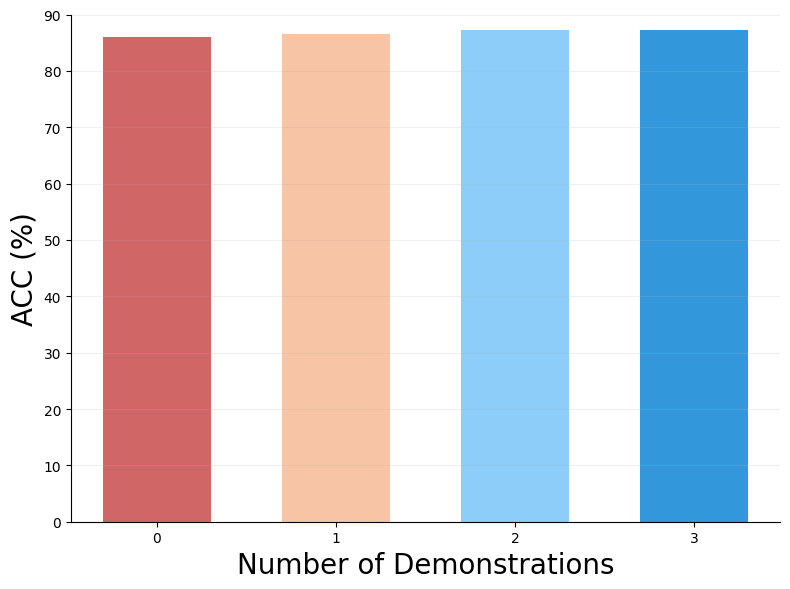
\includegraphics[width=\linewidth]{pics/few_shot.png}
  \caption{Study on Demo Number}
  \label{fig:pnnl1}
\end{subfigure}
\hfill  % Maximize horizontal separation
\begin{subfigure}[t]{0.23\textwidth}  % Top-aligned, 48% of column width
  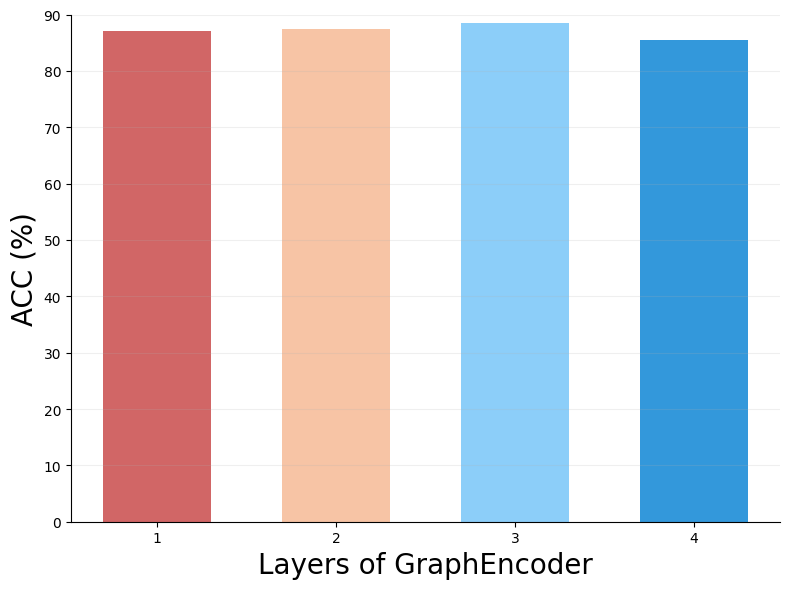
\includegraphics[width=\linewidth]{pics/layer.png}
  \caption{Study on GNN's Layers}
  \label{fig:pnnl2}
\end{subfigure}
\vspace{-0.5\baselineskip}  % Tighter vertical spacing
\caption{Ablation study.}
\label{filtering}
\vspace{-1\baselineskip}  % Tighter vertical spacing
\end{figure}

% For the ablation study, we examine how varying the number of few-shot examples affects model performance. Specifically, we evaluate the accuracy of \myModel{} under zero-shot, 1-shot, 2-shot, and 3-shot settings. Due to the large size of the subgraphs retrieved for SceneGraphs and WebQSP, which exceed the maximum input length supported by the LLM, we conduct the few-shot experiments only on ExplaGraphs. As shown in Figure~\ref{fig:pnnl1}, \myModel{} achieves its best performance with 2-shot learning, while the performance of 2-shot and 3-shot learning is very similar.

% In the hyperparameter study, we explore how the number of layers in the GraphEncoder influences performance. Results, presented in Figure~\ref{fig:pnnl2}, indicate that using three layers achieves the best accuracy across datasets. Deeper configurations (e.g., 4 or more layers) do not yield further gains and may even lead to overfitting. These findings underscore the importance of carefully tuning encoder depth to optimize reasoning performance in \myModel.

We first evaluate how the number of few-shot examples affects \myModel{}'s performance under zero-shot, 1-shot, 2-shot, and 3-shot settings. Since subgraphs in SceneGraphs and WebQSP exceed the LLM's input limit, we perform this study only on ExplaGraphs. As shown in Figure~\ref{fig:pnnl1}, 2-shot learning yields the best performance, with 2-shot and 3-shot results being nearly identical.

In the hyperparameter study, we assess how the number of GraphEncoder layers impacts performance. As shown in Figure~\ref{fig:pnnl2}, using three layers achieves the highest accuracy. Adding more layers offers no further improvement and can cause overfitting. These results highlight the importance of tuning encoder depth for optimal reasoning in \myModel{}.


